%!TEX TS-program = xelatex
\documentclass[12pt, a4paper]{article}\usepackage[]{graphicx}\usepackage[]{color}
%% maxwidth is the original width if it is less than linewidth
%% otherwise use linewidth (to make sure the graphics do not exceed the margin)
\makeatletter
\def\maxwidth{ %
  \ifdim\Gin@nat@width>\linewidth
    \linewidth
  \else
    \Gin@nat@width
  \fi
}
\makeatother

\definecolor{fgcolor}{rgb}{0.345, 0.345, 0.345}
\newcommand{\hlnum}[1]{\textcolor[rgb]{0.686,0.059,0.569}{#1}}%
\newcommand{\hlstr}[1]{\textcolor[rgb]{0.192,0.494,0.8}{#1}}%
\newcommand{\hlcom}[1]{\textcolor[rgb]{0.678,0.584,0.686}{\textit{#1}}}%
\newcommand{\hlopt}[1]{\textcolor[rgb]{0,0,0}{#1}}%
\newcommand{\hlstd}[1]{\textcolor[rgb]{0.345,0.345,0.345}{#1}}%
\newcommand{\hlkwa}[1]{\textcolor[rgb]{0.161,0.373,0.58}{\textbf{#1}}}%
\newcommand{\hlkwb}[1]{\textcolor[rgb]{0.69,0.353,0.396}{#1}}%
\newcommand{\hlkwc}[1]{\textcolor[rgb]{0.333,0.667,0.333}{#1}}%
\newcommand{\hlkwd}[1]{\textcolor[rgb]{0.737,0.353,0.396}{\textbf{#1}}}%
\let\hlipl\hlkwb

\usepackage{framed}
\makeatletter
\newenvironment{kframe}{%
 \def\at@end@of@kframe{}%
 \ifinner\ifhmode%
  \def\at@end@of@kframe{\end{minipage}}%
  \begin{minipage}{\columnwidth}%
 \fi\fi%
 \def\FrameCommand##1{\hskip\@totalleftmargin \hskip-\fboxsep
 \colorbox{shadecolor}{##1}\hskip-\fboxsep
     % There is no \\@totalrightmargin, so:
     \hskip-\linewidth \hskip-\@totalleftmargin \hskip\columnwidth}%
 \MakeFramed {\advance\hsize-\width
   \@totalleftmargin\z@ \linewidth\hsize
   \@setminipage}}%
 {\par\unskip\endMakeFramed%
 \at@end@of@kframe}
\makeatother

\definecolor{shadecolor}{rgb}{.97, .97, .97}
\definecolor{messagecolor}{rgb}{0, 0, 0}
\definecolor{warningcolor}{rgb}{1, 0, 1}
\definecolor{errorcolor}{rgb}{1, 0, 0}
\newenvironment{knitrout}{}{} % an empty environment to be redefined in TeX

\usepackage{alltt}

%%%%%%%%%% Математика %%%%%%%%%%
\usepackage{amsmath,amsfonts,amssymb,amsthm,mathtools}

%%%%%%%%%%%%%%%%%%%%%%%% Шрифты %%%%%%%%%%%%%%%%%%%%%%%%%%%%%%%%%
\usepackage{fontspec}         % пакет для подгрузки шрифтов
\setmainfont{Arial}   % задаёт основной шрифт документа

% Чтобы пропечатывались длинные тире, непрерывные пробелы и тп
\defaultfontfeatures{Mapping=tex-text}

% why do we need \newfontfamily:
% http://tex.stackexchange.com/questions/91507/
\newfontfamily{\cyrillicfonttt}{Arial}
\newfontfamily{\cyrillicfont}{Arial}
\newfontfamily{\cyrillicfontsf}{Arial}

\usepackage{unicode-math}     % пакет для установки математического шрифта
\setmathfont{Asana Math}      % шрифт для математики
% \setmathfont[math-style=ISO]{Asana Math}
% Можно делать смену начертания с помощью разных стилей

% Конкретный символ из конкретного шрифта
% \setmathfont[range=\int]{Neo Euler}

\usepackage{polyglossia}      % Пакет, который позволяет подгружать русские буквы
\setdefaultlanguage{russian}  % Основной язык документа
\setotherlanguage{english}    % Второстепенный язык документа
% Разные мелочи для русского языка из пакета babel
\setkeys{russian}{babelshorthands=true}


\usepackage[paper=a4paper,top=13.5mm, bottom=13.5mm, left=16.5mm, right=13.5mm, includefoot]{geometry}
\usepackage[unicode,colorlinks=true,urlcolor=blue,hyperindex,breaklinks]{hyperref}

\usepackage{indentfirst} % установка отступа в первом абзаце главы!!!
\usepackage{booktabs} 
\usepackage{float}


\title{Отчёт о проделанной работе}
\author{Винни-Пух}
\date{\today}
\IfFileExists{upquote.sty}{\usepackage{upquote}}{}
\begin{document}

\maketitle

\section{Основовы}




\section{Первый чанк или четыре лапки равно собачка}

Тут можно писать текст, и даже вот такие вот формулы

\[ \int_{0}^{+\infty} x^{s-1} \cdot e^{-x} dx = \Gamma(s). \]

Всё совсем как в \LaTeX! Но у нас нет на это времени! Пора создавать чанк!


\begin{knitrout}
\definecolor{shadecolor}{rgb}{0.969, 0.969, 0.969}\color{fgcolor}\begin{kframe}
\begin{alltt}
\hlstd{x} \hlkwb{<-} \hlkwd{rnorm}\hlstd{(}\hlnum{100}\hlstd{)}
\hlstd{x_mean} \hlkwb{<-} \hlkwd{mean}\hlstd{(x)}
\hlstd{x_mean}
\end{alltt}
\begin{verbatim}
## [1] -0.0420707
\end{verbatim}
\end{kframe}
\end{knitrout}

Мы видим, что наши вычисления прошли усспешно и среднее составило -0.0420707



\section{Картинки, таблицы и другие штуки!}




\begin{table}[h!]
\begin{center}

\begin{tabular}{l|r|r|r|r}
\hline
t & GOOG.Open & GOOG.High & GOOG.Low & GOOG.Close\\
\hline
2016-01-04 & 743.00 & 744.060 & 731.258 & 741.84\\
\hline
2016-01-05 & 746.45 & 752.000 & 738.640 & 742.58\\
\hline
2016-01-06 & 730.00 & 747.180 & 728.920 & 743.62\\
\hline
2016-01-07 & 730.31 & 738.500 & 719.060 & 726.39\\
\hline
2016-01-08 & 731.45 & 733.230 & 713.000 & 714.47\\
\hline
2016-01-11 & 716.61 & 718.855 & 703.540 & 716.03\\
\hline
\end{tabular}


\caption{Стоимость акций}
\end{center} 
\end{table}


Таблицы можно получать немного иначе. С помощью пакета xtable. Посмотрим как! Оценим модель с помощью следующего кода: 

\begin{knitrout}
\definecolor{shadecolor}{rgb}{0.969, 0.969, 0.969}\color{fgcolor}\begin{kframe}
\begin{alltt}
\hlstd{formula} \hlkwb{=} \hlstr{"GOOG.Open~t+GOOG.Close"}
\hlstd{model} \hlkwb{<-} \hlkwd{lm}\hlstd{(}\hlkwc{data}\hlstd{=df,formula)}
\end{alltt}
\end{kframe}
\end{knitrout}


Оценки, которые мы заслужили приведены в таблице \ref{tab:regress}. 

% latex table generated in R 3.3.2 by xtable 1.8-2 package
% Thu Mar 23 12:36:10 2017
\begin{table}[ht]
\centering
\begin{tabular}{rrrrr}
  \hline
 & Estimate & Std. Error & t value & Pr($>$$|$t$|$) \\ 
  \hline
(Intercept) & 302.96 & 181.98 & 1.66 & 0.10 \\ 
  t & -0.02 & 0.01 & -1.48 & 0.14 \\ 
  GOOG.Close & 0.96 & 0.03 & 33.22 & 0.00 \\ 
   \hline
\end{tabular}
\caption{Оценки, которые мы заслужили!} 
\label{tab:regress}
\end{table}



% latex table generated in R 3.3.2 by xtable 1.8-2 package
% Thu Mar 23 12:37:05 2017
\begin{table}[ht]
\centering
\begin{tabular}{rrrrr}
  \hline
 & Estimate & Std. Error & t value & Pr($>$$|$t$|$) \\ 
  \hline
(Intercept) & 302.96 & 181.98 & 1.66 & 0.10 \\ 
  t & -0.02 & 0.01 & -1.48 & 0.14 \\ 
  GOOG.Close & 0.96 & 0.03 & 33.22 & 0.00 \\ 
   \hline
\end{tabular}
\caption{Оценки, которые мы заслужили!} 
\label{tab:regress}
\end{table}


Графики можно построить совсем разными. Например, вот такой! 


\begin{knitrout}
\definecolor{shadecolor}{rgb}{0.969, 0.969, 0.969}\color{fgcolor}

{\centering 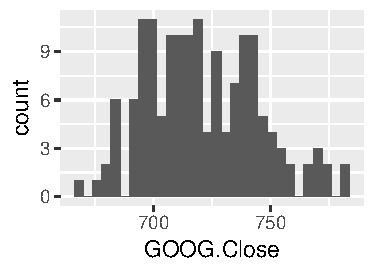
\includegraphics[width=\maxwidth]{figure/unnamed-chunk-7-1} 

}



\end{knitrout}

Можно к коду использовать любые окружения теха! Прямо как к рисунку \ref{fig}.

\begin{figure}[h!]
\begin{knitrout}
\definecolor{shadecolor}{rgb}{0.969, 0.969, 0.969}\color{fgcolor}

{\centering 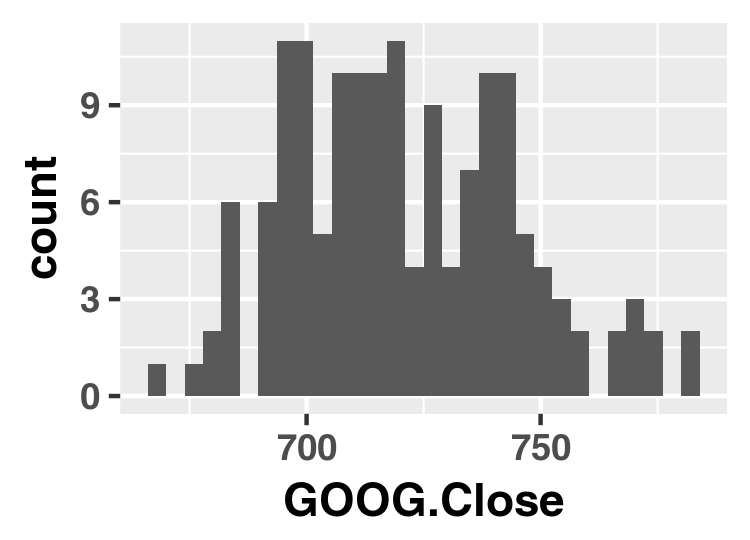
\includegraphics[width=\maxwidth]{figure/unnamed-chunk-8-1} 

}



\end{knitrout}
\caption{Гистограмка для стоимости акций гугл! \label{fig}}
\end{figure}


Средняя цена заыкрытия акции гугла рана $720.7921207$

Команда \$ \$ делает в техе формулу. Команда Sexpr обращается к R. Все, что написано в скобках к Sexpr будет посчитано в R и вставленно в \TeX. 


\section{Имена чанков}

Чанкам можно давать имена! Напримеп, ниже чанк по имени Антон. Зачем их давать? Это забавно. Да и ктому же чанки удобно искать по именам...




\end{document}
